\documentclass[12pt]{article}
\usepackage{setspace}   % paquete para interlineado
\usepackage{newtxtext,newtxmath} % Times New Roman

%otra opcion para times roman adaptable a versiones
%\usepackage{mathptmx}

%haber si funciona mas parecido a word
\setstretch{1.5}  
%\usepackage[protrusion,expansion]{microtype}
%\onehalfspacing               % interlineado 1.5
\usepackage{amsmath} % Para usar \text{}
\usepackage[utf8]{inputenc}
\usepackage[spanish]{babel}
\usepackage[letterpaper, left=3cm, right=2.5cm, top=2.5cm, bottom=2.5cm]{geometry}
\usepackage{graphicx}
\usepackage{titlesec}
\usepackage{setspace}
\usepackage{lipsum}
\geometry{margin=1in}


%%.......NUEVO-------------%%
\usepackage{longtable}   % tablas que se parten entre páginas




%%%-------------nuevos-----------%%%%%%%%%%
% === Paquetes extra para tablas y utilidades ===
\usepackage{tabularx}   % tablas que se ajustan al ancho
\usepackage{booktabs}   % reglas de tabla profesionales
\usepackage{array}      % nuevas columnas tipo m{..}, p{..}
\usepackage{multirow}   % celdas combinadas verticalmente
\usepackage{xcolor}     % (opcional) para resaltar si lo deseas
\usepackage{hyperref}   % ya lo usas a veces: enlaces internos/TOC

% === Macros útiles del checklist ===
\newcommand{\cbox}{\(\square\)}       % casilla vacía






%PAQUETE para incluir PDF´s
\usepackage{pdfpages} % para incluir PDFs

% ---PAQUETE PARA contador para las introducciones ---
\newcounter{intro}
\renewcommand{\theintro}{\arabic{intro}} % numeración arábiga: 1,2,3,...


% PAQUETE PARA COMENTAR FACILMENTE 

\usepackage{comment}

%%FORZAR LAS IMAGENES CON FLOAT

\usepackage{float} % necesario para usar [H]


% ESPACION DE TITULOS*{comando}{margen_izq}{espacio_antes}{espacio_despues}
%\titlespacing*{\section}
%{0pt}    % sangría izquierda
%{3em}    % espacio ANTES del título
%{0em}    % espacio después del título




 % PAQUETE PARA INSTANCIAR  LAS IMAGENES
  \graphicspath{{./Imagenes}}
 

%CONFIGURACION DE MI PAGINA numeración:
%\usepackage{fancyhdr}
%\pagestyle{fancy}
%\fancyhf{} % Limpia encabezados/pies
%\fancyhead[R]{\thepage} % Números arábigos arriba: izq en pares, der en impares
%\renewcommand{\headrulewidth}{0pt} % Sin línea

%COLOCAR NUMERACION ESQUINA DERECHA PAG 1
%\fancypagestyle{plain}{%
%	\fancyhf{}%
%	\fancyhead[R]{\thepage}%
%	\renewcommand{\headrulewidth}{0pt}%



% --- PAQUETES ADICIONALES DE LOSA ---
  % para listas multinivel (numeración + incisos + viñetas)
\usepackage{enumitem} 

% que los párrafos  de las secciones dentro de los items usen la misma sangría que el cuerpo SANGRIA A TODOWWW
\setlist[enumerate]{listparindent=\parindent, parsep=0pt}

\begin{comment}
	
	% --- Configuración de enumitem para numeración multinivel ---
	\setlist[enumerate,1]{label=\arabic*., leftmargin=1.2cm}
	\setlist[enumerate,2]{label=\arabic{enumi}.\arabic*., leftmargin=1.4cm}
	\setlist[enumerate,3]{label=\arabic{enumi}.\arabic{enumii}.\arabic*., leftmargin=1.6cm}
	\setlist[enumerate,4]{label=\alph*) , leftmargin=1.8cm}
	\setlist[itemize]{leftmargin=1.6cm}
	
\end{comment}


\begin{comment}
	PARA INDICES CREO
	\tableofcontents
	\newpage
\end{comment}



\begin{document}
	
	%Para no generar numeracion de paginas
	\pagestyle{empty}
	
%	\thispagestyle{fancy} 
	
	%es para emparejar el tamaño de todas las letras de titulo y contenido
%	\titleformat{\section}{\large\bfseries}{\thesection.}{0.5em}{}
%	\titleformat{\subsection}{\normalsize\bfseries}{\thesubsection.}{0.5em}{}
	
	%\title{\vspace{-2cm}Área de Métodos Constructivos
%	\\ Descripción y proceso constructivo de losas}
%	\author{}
%	\date{}
	

	
	
	
%	\maketitle
	
	%\vspace{-2.5cm}
	
%
\includepdf{portadaU2/caratulaU}
%
\includepdf[pages=-,pagecommand={}]{hoja/hojaadjunta}

%%-----------TITULOSSSS--------------------------------------
		\begin{center}
		\textbf{\LARGE  Métodos Constructivos}
	\end{center}

%--------------SUBTITULOS---------------------

	% Primera introducción
\stepcounter{intro}
%\section*{\theintro\ Descripción y proceso constructivo de losas}
%\addcontentsline{toc}{section}{\theintro\ Descripción y proceso constructivo de losas}
 

	
%-------------LOSA TRADICIONAAAAL--------------------


\section*{\theintro\ Proceso Constructivo de Losas}
\addcontentsline{toc}{section}{\theintro\ Descripción y proceso constructivo de elementos de concreto}

	
	\section{Losa Concreto Armado}

Las losas de concreto forman la parte más difícil y que al mismo tiempo requiere mas trabajo del proceso constructivo, por lo que deben hacerse en forma cuidadosa con objeto de evitar posibles accidentes motivados por defectos de construccion. Las losas de concreto armado se apoyan sobre muros o vigas. El armado se hace con varilla del número 2 1/2 o del 3.

%\vspace{0.5} % agrega 1 cm de espacio
\begin{figure}[h]
	\centering
	
\includegraphics[width=0.6\textwidth]{imagen1}
	\caption{Proceso de armado con retícula y refuerzos perimetrales}
	\label{fig:losa1}
\end{figure}

\begin{itemize}
	\item Se utilizan en construcciones definitivas en regiones que cuenten con los materiales apropiados para su elaboración: cemento, grava, arena, fierro y cimbra.
	\item Es indispensable contar con mano de obra y supervisión calificadas.
	\item Son muy resistentes, rígidas, aislantes y pueden construirse de la forma que sea necesaria.
	\item Las dimensiones, armados, especificaciones y sistemas constructivos a emplear estarán en los planos estructurales.
\end{itemize}



	\subsection{Paso 1: Cimbrado}
	Antes de tender cualquier armado debe checarse que toda la cimbra este impregnada con aceite Diesel para evitar que se adhiera al concreto; así mismo se vigila que las juntas entre las tablas sean a tope para evitar el escurrimiento del concreto.
	
	
	%\vspace{0.5} % agrega 1 cm de espacio
	\begin{figure}[h]
		\centering
		
\includegraphics[width=0.6\textwidth]{imagen2}
			\caption{Limpieza de terreno}
		\label{fig:losa2}
	\end{figure}
	
	%-----------------------------
	
	\subsection{Paso 2: Armado}
	\begin{itemize}
		\item Se revisa la correcta posición del armado.
		\item Las varillas se amarran en todos sus cruces y se vigila el correcto empleo de silletas para que las varillas queden perfectamente ahogadas y con el recubrimiento adecuado.
	\end{itemize}
	
	
	
	

	
	\begin{figure}[h!]
		\centering
		
\includegraphics[width=0.6\textwidth]{imagen3}
		\caption{Materiales y herramientas}
		\label{fig:losa3}
	\end{figure}
	
	%---------------------------------
	
	
	\subsection{Paso 3: Fabricación del concreto}
	
	\begin{itemize}
		\item Se calcula la proporción de cada material según la resistencia deseada (por ejemplo, \(f'_c = 210~\text{kg/cm}^2\) o \(280~\text{kg/cm}^2\)).
		\item Una dosificación típica para concreto estructural puede ser:
		\begin{itemize}
			\item 1 parte de cemento
			\item 2 partes de arena
			\item 3 partes de grava
			\item 0.5 partes de agua
		\end{itemize}
	\end{itemize}
	
		\begin{figure}[h!]
		\centering
		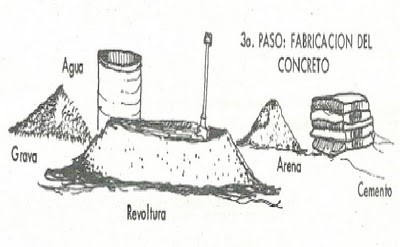
\includegraphics[width=0.6\textwidth]{imagen4}
		\caption{Materiales y herramientas}
		\label{fig:losa3}
	\end{figure}
	
		%---------------------------------
	
	
	\subsection{Paso 4: Colado}
	
	\begin{itemize}
		\item Si se emplea en el colado concreto normal se descimbrará 15 días después de vaciado el concreto, vigilando que queden puntales o pies derechos hasta completar 28 días.
		\item En losas de concreto pueden hacerse huecos o perforaciones de cualquier tamaño si se toman las medidas adecuadas para absorber los esfuerzos producidos.
	\end{itemize}
	
	\begin{figure}[h!]
		\centering
		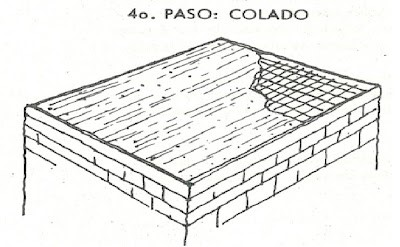
\includegraphics[width=0.6\textwidth]{imagen5}
		\caption{Materiales y herramientas}
		\label{fig:losa3}
	\end{figure}
	
		%---------------------------------
	
	
	\subsection{Paso 5: Curado y descimbrado:}
	
	\begin{itemize}
		\item Una vez que se ha realizado todo el colado, debe procederse al curado, que consiste en mojar la superficie de la losa dos o tres veces al dia durante un periodo de una semana.
		\item Esto tiene por objeto evitar que la losa se agriete por perdida excesiva del agua del concreto.
		\item A partir del dia siguiente de efectuado el colado se cura la losa regándola con agua durante una semana, tres veces al dia esto para evitar el agrietamiento de la losa.
		
	\end{itemize}
	
	\begin{figure}[h!]
		\centering
		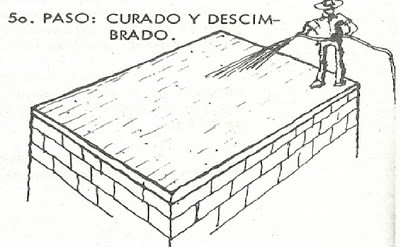
\includegraphics[width=0.6\textwidth]{imagen6}
		\caption{Materiales y herramientas}
		\label{fig:losa3}
	\end{figure}
	
	
		%---------------------------------
	
	
	\subsection{Elementos del Armado de una Losa: Columpios, Bastones y Varillas Rectas}
	
	\begin{itemize}
		\item El armado de una losa necesita de columpios, bastones y varillas rectas, y el alambre recocido del numero 18 para amarrar los cruces.
	
		
	\end{itemize}
	
	\begin{figure}[h!]
		\centering
		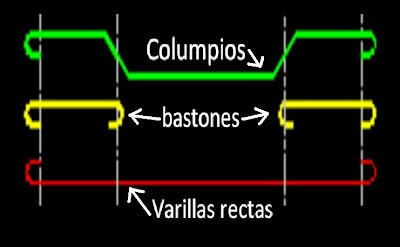
\includegraphics[width=0.6\textwidth]{imagen7}
		\caption{Materiales y herramientas}
		\label{fig:losa3}
	\end{figure}
	
	
	\subsubsection{Pasos para hacer el armado de una losa:}
	
	\begin{itemize}
		\item Poner varillas rectas tanto en el sentido vertical como en el horizontal, espaciadas entre 15 y 25 centímetros. Estas varillas se amarran en sus cruces con alambre recocido del \#18.
		\item Entre cada varilla recta, poner un columpio en ambos sentidos. Amarrar en los cruces.
		\item Entre cada columpio se colocan los bastones, amarrando también en los cruces.
	\end{itemize}
	
		\begin{figure}[H]
		\centering
		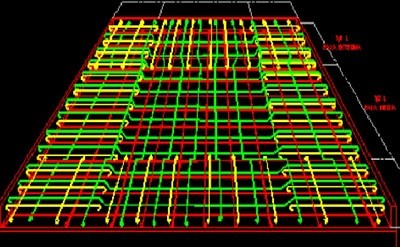
\includegraphics[width=0.6\textwidth]{imagen8}
		\caption{Materiales y herramientas}
		\label{fig:losa3}
		\end{figure}
	

	

	
	%-----------------------------------------------------------
	
	
	\section{Vigueta y bovedilla}
	
	\subsection*{Pasos de ejecución (paso a paso)}
	\begin{enumerate}
		\item \textbf{Replanteo y revisión de apoyos.} Verificar claros, alineación de muros o vigas y que exista el \emph{apoyo mínimo} para cada vigueta. El apoyo mínimo típico reportado por fabricantes va desde \textbf{5 cm} hasta \textbf{$\geq$ 9 cm}; utilizar siempre lo indicado por el proveedor y el cálculo estructural del proyecto.
		\item \textbf{Apuntalamiento perimetral y líneas de nivel.} Colocar \textbf{puntales} y \textbf{largueros} para nivelar y sostener durante el montaje y el colado. El sistema reduce o elimina cimbra de contacto, pero \textbf{sí requiere apuntalamiento} para controlar flechas y seguridad.
		\item \textbf{Colocación de viguetas (desde el muro de arranque).} Presentar y apoyar las viguetas en la dala/trabe de apoyo; respetar la \textbf{separación entre ejes} conforme al ancho de bovedilla y los planos. Puede emplearse una \textbf{bovedilla guía} para fijar la distancia correcta entre viguetas.
		\item \textbf{Alineación inicial con bovedillas de borde.} Colocar primero bovedillas en \textbf{orillas/extremos} para escantillar la modulación y ayudar a la \textbf{alineación} de las viguetas antes de llenar el campo.
		\item \textbf{Colocación de bovedillas (campo).} Colocar manualmente las bovedillas \textbf{juntas y bien apoyadas} sobre las alas de las viguetas; avanzar de un extremo al otro utilizando tablones de paso para distribuir cargas.
		\item \textbf{Paso y protección para instalaciones.} Prever \textbf{ductos eléctricos}, salidas y pasos sanitarios \textbf{antes} de la malla y la capa de compresión. Donde se retire una bovedilla para una salida o registro, \textbf{cimbrar inferiormente} y \textbf{reforzar} conforme a los planos.
		\item \textbf{Refuerzos locales y armados adicionales (si aplica).} Colocar \textbf{refuerzos en apoyos/claros} (armaduras negativas, nervaduras de amarre, bastones u otros) cuando lo especifique el diseño estructural o el proveedor del sistema.
		\item \textbf{Malla electrosoldada y traslapes.} Tender la \textbf{malla} sobre toda la losa; realizar \textbf{traslapes} típicos de \textbf{10--15 cm} y sujetar con alambre. Es \textbf{crítico} que la malla quede \textbf{totalmente dentro de la capa de compresión} (emplear calces/silletas adecuados).
		\item \textbf{Preparación para colado (humedecido).} \textbf{Humedecer} viguetas y bovedillas antes del colado para mejorar la adherencia y reducir succión (en bovedillas cerámicas o porosas se recomienda saturar bien).
		\item \textbf{Colado de la capa de compresión.} Espesor típico \textbf{$\geq$ 4--5 cm} (o el indicado en planos, pudiendo ser \textbf{5--6 cm} según material de bovedilla y peraltes). Usar concreto de calidad estructural acorde al proyecto. Iniciar el vaciado en \textbf{dalas/trabes} y continuar \textbf{de bordes hacia el centro}, evitando descargar en un solo punto; \textbf{vibrar/lanear} para eliminar oquedades y lograr nivel.
		\item \textbf{Curado.} Mantener la losa \textbf{húmeda} al menos \textbf{7 días} (o según especificación/NTC) para controlar fisuración por retracción y asegurar el desarrollo de resistencia.
		\item \textbf{Retiro de apuntalamientos.} Desencofrar/retirar puntales \textbf{cuando el concreto alcance la resistencia requerida} y según el \textbf{criterio del proyecto y/o proveedor}. Considerar ambiente, temperatura, tipo de cemento y tiempos de fraguado.
	\end{enumerate}
	

	
	
	
	

	

	
	%------------------------------------------------------------
	
	
	
	
	
	
	
	
	
	
	%---------------LOSA NERVADA--------------------
	\section{Losa nervada }
	
	
	La \textbf{losa nervada} es un sistema bidireccional formado por una malla de \textbf{nervaduras} (trabes perpendiculares entre sí) y una \textbf{losa de compresión} superior. Los \textbf{casetones} o elementos de aligeramiento (plástico, poliestireno, fibrocemento o prefabricados) generan vacíos entre nervaduras para \textbf{reducir peso propio} sin perder rigidez. Se emplea en claros medianos a grandes, cuando se busca \textbf{ahorro de material} y buen \textbf{comportamiento bidireccional}.
	
	\subsection{Proceso constructivo (paso a paso)}
	\begin{enumerate}
		\item \textbf{Replanteo y cimbra.} Trazar ejes, claros y peraltes según planos. Colocar \textbf{cimbra base} perfectamente nivelada y apuntalamientos con la separación indicada para controlar flechas durante colado.
		\item \textbf{Colocación de casetones/aligerantes.} Instalar los casetones conforme a la \textbf{modulación} del proyecto (cuadriculado). Asegurarlos para evitar flotación o desplazamientos durante el vaciado.
		\item \textbf{Armaduras en nervaduras.} Colocar el \textbf{acero inferior y superior} de las nervaduras (negativos en apoyos si aplica), ganchos, estribos y traslapes según el detalle estructural. Verificar recubrimientos con calces/silletas.
		\item \textbf{Armadura de la losa de compresión.} Tender \textbf{malla electrosoldada} o varillas superiores con traslapes adecuados, garantizando que queden \textbf{embebidos} dentro del espesor de la capa de compresión.
		\item \textbf{Instalaciones y huecos.} Definir pasos de instalaciones (eléctricas, sanitarias, HVAC) \textbf{antes} del colado. Donde haya huecos, disponer \textbf{cimbra localizada} y refuerzos perimetrales según planos.
		\item \textbf{Revisión de niveles y limpieza.} Confirmar peraltes, recubrimientos, líneas de nivel y limpieza de la cimbra/casetones para favorecer la adherencia del concreto.
		\item \textbf{Colado de nervaduras y losa de compresión.} Vaciar concreto de la \textbf{resistencia especificada}, preferentemente de manera continua: primero llenar \textbf{nervaduras} y luego la \textbf{capa de compresión} (espesor típico de proyecto, p.\,ej. 4--6\,cm). Vibrar/lanear sin desplazar armados o casetones.
		\item \textbf{Curado.} Mantener la losa \textbf{húmeda} el tiempo indicado (p.\,ej. \(\geq\) 7 días) para controlar fisuración y asegurar el desarrollo de resistencia.
		\item \textbf{Descimbrado y retiro de casetones (si son recuperables).} Retirar de forma \textbf{progresiva} cuando el concreto alcance la resistencia requerida. Si los casetones son recuperables, desmontarlos con cuidado y limpiar para su reutilización.
		\item \textbf{Acabados y control final.} Verificar flechas, regularidad de nervaduras, planicidad y dimensiones de casetones visibles; proceder con acabados según especificación.
	\end{enumerate}
	

	

	%----------------------------------------------
	
	
	

	
		
	
	%---------------------------------------------------
	

	
	\section{Losacero}

	Por regla general, a la hora de construir edificaciones o estructuras, hay dos aspectos que se buscan lograr al máximo: calidad y costo accesible. Para alcanzar esos estándares, la industria de la construcción ofrece muchas opciones.
		
	Entre todas estas, se debe evaluar qué materiales funcionan mejor para cada tipo de construcción, tomando en cuenta el terreno donde se realiza la obra o el nivel de seguridad que debe tener una edificación, según las condiciones ambientales.
	
	
	El sistema losacero es una opción de construcción que ofrece seguridad y solidez para muchos proyectos, además de ser un sistema estructural excelente.
	
	
	\subsection{¿Qué es losacero?}
	
	El sistema losacero es un entrepiso metálico que cuenta con un perfil laminado que interactúa con el concreto para brindar solidez y resistencia estructural a losas de edificios y otro tipo de construcciones.
	
	
	\begin{figure}[h]
		\centering
		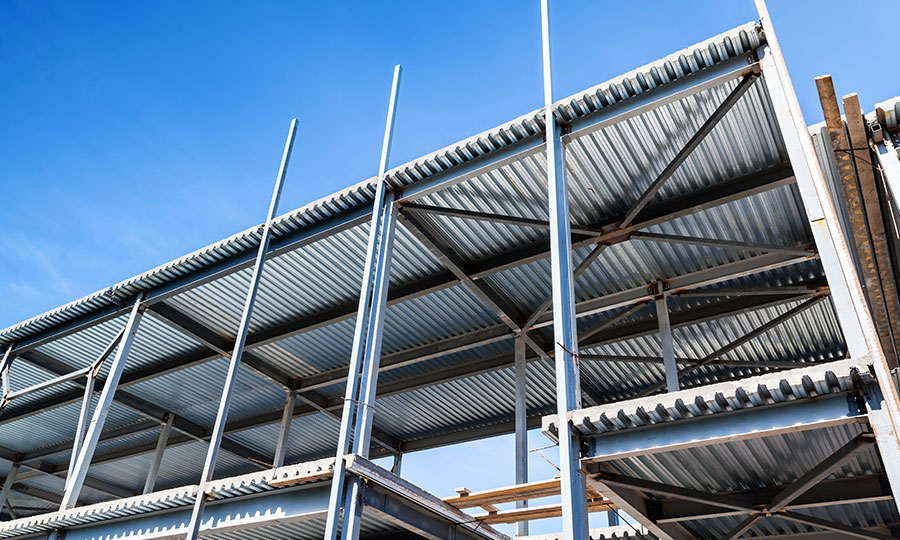
\includegraphics[width=0.7\textwidth]{losacero-1.jpg}
		\caption{sistema losacero PSI Concreto}
	\end{figure}
	
\begin{itemize}
	\item El sistema losacero ofrece seguridad, resistencia y varios beneficios para la construcción de edificaciones de distintos tipos.
	

	\item Según el Steel Deck Institute, el losacero tiene tres funciones principales: actuar como plataforma de trabajo durante la construcción, proveer refuerzo positivo por flexión a la losa de concreto y otorgar resistencia para cargas horizontales.
\end{itemize}


\subsection{Pasos de ejecución (paso a paso)}
\begin{enumerate}
	\item \textbf{Replanteo y preparación de apoyos.} Verificar claros, ejes y alineación de vigas/estructuras de acero que recibirán la lámina acanalada (losacero). Confirmar cotas, niveles y que las superficies de apoyo estén limpias y libres de rebabas u obstáculos.
	\item \textbf{Apuntalamientos provisionales (si aplica).} Colocar puntales o sopandas temporales bajo los paños de mayor claro cuando así lo requiera el cálculo, para controlar flechas durante el colado y la etapa fresca del concreto.
	\item \textbf{Colocación de la lámina losacero.} Tender los paneles de lámina acanalada en el sentido indicado por proyecto, apoyándolos sobre vigas secundarias/principales. Presentar la primera lámina como referencia y continuar con las siguientes manteniendo modulación y plomos.
	\item \textbf{Traslapes longitudinales y transversales.} Ejecutar los traslapes entre paneles conforme a la geometría del perfil (cresta/valle) y al detalle de proyecto; asegurar continuidad y estanqueidad para evitar filtraciones de lechada durante el colado.
	\item \textbf{Fijación mecánica a la estructura.} Anclar la lámina a vigas y correas mediante tornillos autoperforantes, clavos de pólvora o sistemas equivalentes, con el \emph{paso} y patrón de fijación especificado (borde y campo). Comprobar que no existan láminas flojas o con juego.
	\item \textbf{Conectores de cortante (si es sistema colaborante).} Soldar o instalar \emph{studs} conectores sobre las vigas de acero atravesando la lámina, con la separación y diámetro de proyecto. Verificar penetración, verticalidad y ausencia de soldaduras frías.
	\item \textbf{Cierres perimetrales y diafragmas.} Colocar ángulos, soleras o piezas de cierre en perímetros, huecos y juntas; instalar diafragmas o diafragmas de borde si están especificados para transmitir esfuerzos de diafragma al sistema de arriostramiento.
	\item \textbf{Tratamiento de huecos y pasos.} Definir pasos de instalaciones (eléctricas, sanitarias, HVAC) antes del colado. Donde se requieran huecos, colocar moldes o cajas perdidas, y reforzar los bordes del hueco según detalle estructural.
	\item \textbf{Refuerzos locales.} Disponer varillas de refuerzo adicional en apoyos, sobre vigas, en zonas de negativos, al pie de huecos y en cambios de sección conforme a planos; amarrar con alambre recocido para evitar desplazamientos durante el colado.
	\item \textbf{Malla electrosoldada y calces.} Tender la malla electrosoldada sobre la losa, con traslapes adecuados y sujeción puntual. Colocar \emph{silletas} o calces para garantizar que la malla quede completamente embebida dentro de la capa de compresión, a la altura indicada.
	\item \textbf{Bordillos, juntas y nivelación.} Instalar tableros de borde, juntas de construcción o de dilatación según corresponda; verificar pendientes y referencias de nivel (reglas/maestros) para el acabado final de la losa.
	\item \textbf{Colado de la capa de compresión.} Humedecer previamente la lámina y la superficie; colar el concreto con revenimiento y resistencia especificados, distribuyendo de manera uniforme, sin sobrecargar un punto. Vibrar o lanear lo necesario para eliminar oquedades y lograr un acabado nivelado.
	\item \textbf{Curado.} Iniciar el curado tan pronto lo permita la superficie, manteniendo la humedad el tiempo indicado para controlar retracción plástica y asegurar el desarrollo de resistencia. Proteger la losa del sol y viento excesivos.
	\item \textbf{Retiro de apuntalamientos y limpieza.} Retirar los apuntalamientos provisionales cuando el concreto alcance la resistencia requerida por el proyecto. Limpiar la zona de trabajo y verificar que no existan elementos sueltos o proyecciones de concreto que interfieran con acabados posteriores.
\end{enumerate}



	%-----------------------------------------------------








	
	%--------------SUBTITULOS 2---------------------
	
	% Segunda introducción
	\stepcounter{intro}
	\section*{\theintro\ Proceso constructivo de elementos de concreto}
	\addcontentsline{toc}{section}{\theintro\ Descripción y proceso constructivo de elementos de concreto}
	
	%REINICIAR CONTEO DE SECTION 
	\setcounter{section}{0}
		
	\section{Levantado de muros de Mampostería}
	El levantado de muros de mampostería es el proceso constructivo mediante el cual se construyen los muros de un edificio u obra utilizando unidades de mampostería (bloques de concreto, ladrillos de arcilla, piedra, entre otros) unidas con mortero.
	
	Así también consiste en disponer ordenadamente las unidades de mampostería en hiladas horizontales, siguiendo un trazo y plomo definidos, y asegurando que cada unidad quede ligada a las demás mediante mortero de pega. El levantado no se limita a “poner blocks”, sino que incluye la verificación de alineaciones, niveles, juntas llenas y continuidad estructural.
	
	\textbf{Características principales}:
	\begin{itemize}
		\item \textbf{Materiales}: bloques o ladrillos, mortero de pega y, en muchos casos, refuerzo (acero y graut).
		\item \textbf{Orden constructivo}: se inicia sobre la cimentación o sobre una solera de arranque, asegurando que la primera hilada quede perfectamente nivelada.
		\item \textbf{Juntas}: las horizontales y verticales deben quedar totalmente llenas de mortero para garantizar adherencia y estabilidad.
		\item \textbf{Refuerzo y confinamiento}: en sistemas sismorresistentes como los que regulan las NSE de Guatemala, el levantado incluye la previsión de columnetas, soleras y grauteo de celdas donde van alojadas las varillas.
	\end{itemize}
	
		\begin{figure}[h]
		\centering
		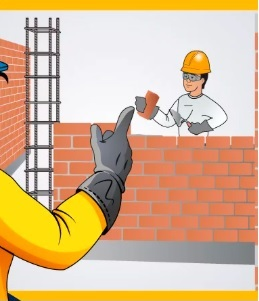
\includegraphics[width=0.4\textwidth]{mampos1}
		\caption{Muro de Mampostería}
		\end{figure}
	
	
		
	\subsection{Proceso constructivo}
	\subsubsection{Preparación y replanteo}
	\begin{enumerate}
		\item Revisión de planos y memorias conforme NSE 1 y NSE 7.4 (dimensiones, ubicación de columnetas/mochetas, soleras, vanos, cuantías). Registrar supervisión técnica.
		\item Cimentación y arranques listos (plomos de control). Nivelar y trazar ejes de muros y vanos.
		\item Unidades de mampostería (block/ladrillo) conformes a proyecto; verificar resistencia de unidades y f´m de la mampostería según tablas/criterios de la norma.
	\end{enumerate}
	
	\subsubsection{Mortero de pega}
	\begin{enumerate}
		\item Seleccionar tipo de mortero (p. ej. Tipo S o N, según exposición/cargas) y proporciones por desempeño conforme NTG 41050 (ASTM C270).
		\item Mezclado: materiales limpios, dosificación consistente; evitar exceso de agua.
		\item Controlar retención de agua y trabajabilidad (adherencia) según clima y succión de las unidades.
	\end{enumerate}
	
			
	\begin{figure}[h]
		\centering
		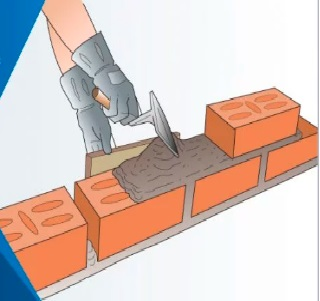
\includegraphics[width=0.4\textwidth]{mampos2}
		\caption{Distribución de mezcla}
	\end{figure}
		
	
	\subsubsection{Colocación de hiladas}
	\begin{enumerate}
		\item Primera hilada sobre mortero nivelado; controlar plomo, nivel y alineación.
		\item Espesor de juntas típico de 10 mm y llenado continuo.
		\item Minimizar el tiempo entre extender mortero y asentar la unidad (ideal $<$1 min) para no perder adhesión por succión/evaporación.
		\item Humedecido previo: si la unidad tiene alta succión, humedecer moderadamente; si es de muy baja succión, aumentar tiempo antes de asentar para evitar “flotación”.
	\end{enumerate}
	
		
	\begin{figure}[h]
		\centering
		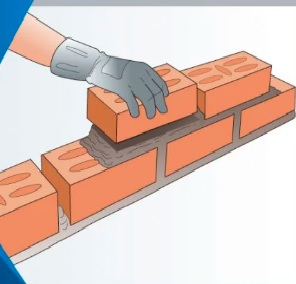
\includegraphics[width=0.4\textwidth]{mampos4}
		\caption{Colocación de ladrillo}
	\end{figure}
	
	
	
	\subsubsection{Armado y elementos de confinamiento}
	\begin{enumerate}
		\item Sistema confinado: muros con columnetas/mochetas y soleras de concreto que confinan el paño; es la modalidad prioritaria en Guatemala.
		\item Refuerzo en juntas de mortero no se reconoce con función estructural en la NSE 7.4.
		\item Columnetas: respetar límites de dimensiones y cuantías mínimas verticales ($\rho \geq 0.0075$, $\leq 0.02$) y mínimo 8 barras longitudinales con estribos adecuados.
		\item Dinteles y soleras: diseñar/armar según criterio de resistencia a corte y flexión, espaciamiento máximo de barras a flexión y, cuando aplique, refuerzo de corte; controlar deflexión y compatibilidad con la respuesta sísmica del marco/muro.
		\item Anclajes/pases: prever varillas, conectores, paso de instalaciones sin debilitar el diafragma del muro; coordinar con NSE-3.
	\end{enumerate}
	
	\subsubsection{Inyección (grauteo)}
	\begin{enumerate}
		\item Graut: elegir fino o grueso; convencional (asentamiento 200–280 mm) o autoconsolidante (flujo 610–760 mm; VSI $\leq$ 1), siempre con f’c $\geq$ 14 MPa a 28 días.
		\item Colocación por etapas: vibrado/varillado en graut convencional; continuidad entre levantados; no dejar “cuellos fríos”.
		\item Control de altura de levantado por jornada según especificación y práctica de obra.
	\end{enumerate}
	
	\subsubsection{Aperturas y remates}
	\begin{enumerate}
		\item Vanos con dinteles conformes a NSE 7.4; respetar apoyos mínimos, continuidad de soleras y confinamiento.
		\item Evitar concentrar instalaciones cerca de esquinas de vanos.
	\end{enumerate}
	
	\subsection{Curado y protección}
	\begin{itemize}
		\item Mortero (juntas): proteger del viento/sol para reducir evaporación; mantener humedad inicial suficiente (niebla ligera/pañete húmedo) sin encharcar.
		\item Graut: mantener condiciones que favorezcan hidratación; evitar lavado por lluvia; en autoconsolidantes, respetar recomendaciones del fabricante y NTG 41052.
		\item Clima:
		\begin{itemize}
			\item En calor/viento usar morteros con alta retención de agua.
			\item En frío llevar materiales $>$0°C antes de pegar, minimizar agua libre y proteger contra congelación.
		\end{itemize}
	\end{itemize}
	
	
		
	\begin{figure}[h]
		\centering
		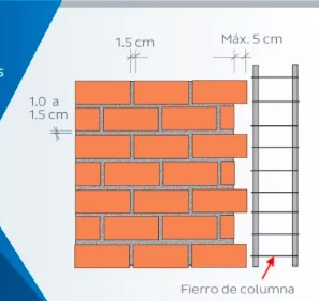
\includegraphics[width=0.4\textwidth]{mampos3}
		\caption{Espesor del mortero entre ladrillos }
	\end{figure}
	
	
	\subsection{Control de calidad y supervisión}
	\begin{itemize}
		\item Supervisión técnica obligatoria (NSE 1): bitácora, presencia en colocación de unidades, armaduras e inyección de graut.
		\item Materiales: verificar certificados de unidades, cemento, agregados; para graut usar NTG 41056 (ASTM C1019) para resistencia de compresión.
		\item Conformidad constructiva: la NSE 7.4 define propiedades geométricas (área neta/efectiva), colocación de lechos de mortero y no reconocer función estructural a varillas en juntas.
	\end{itemize}
	
	\subsection{Ventajas y desventajas}
	\subsubsection{Ventajas}
	\begin{itemize}
		\item Buen desempeño sísmico en vivienda de baja altura cuando se confinan paños y se respetan derivas/detalles (norma local específica).
		\item Disponibilidad de materiales y mano de obra en Guatemala; procesos conocidos.
		\item Rigidez lateral y compartimentación; facilidad para acabados.
		\item Compatibilidad normativa con NSE y referencia a TMS 402/602 para criterios puntuales.
	\end{itemize}
	
	\subsubsection{Desventajas}
	\begin{itemize}
		\item Sensibilidad a la calidad de ejecución (alineación, llenado de juntas y celdas, curado); errores reducen adherencia y capacidad.
		\item Interrupciones por vanos y mal resuelto de dinteles pueden crear debilidades locales si no se siguen los detalles de la NSE 7.4.
		\item Modificaciones posteriores (ranurados, pases) pueden comprometer el confinamiento si no se controlan.
		\item Peso propio mayor que sistemas livianos (implica considerar demanda sísmica conforme NSE-3).
	\end{itemize}
	%%-------------------------------------------------
	
	

	
	
	
	
	
	
	
	%%-------------MOCHETAS------------------------
	
	\section{Mochetas}
	
	La mocheta en mampostería es un elemento constructivo que forma un resalte o saliente en los muros de bloques o ladrillos, y que cumple funciones tanto estructurales como arquitectónicas.
	  
	Arquitectónicamente, se utiliza como acabado lateral de los vanos de puertas y ventanas, brindando mayor espesor y rigidez para recibir marcos, carpintería o cerramientos.  
	
	
	Estructuralmente, la mocheta puede actuar como jamba o elemento de confinamiento, mejorando la resistencia del muro frente a cargas verticales y laterales.  
	- En muchos casos, la mocheta se construye como parte de un sistema de mampostería reforzada, rellenando celdas de bloque con concreto y barras de acero, lo cual la convierte en un elemento capaz de resistir esfuerzos de compresión y cortante.  
	
	Según la NSE 7.4 de AGIES, las mochetas que funcionan como jambas de los vanos deben estar confinadas por soleras y castillos, además de contar con refuerzo vertical continuo. Esto asegura que, en caso de sismo, la apertura de vanos no debilite el muro.  
	 
	\begin{figure}[h]
		\centering
		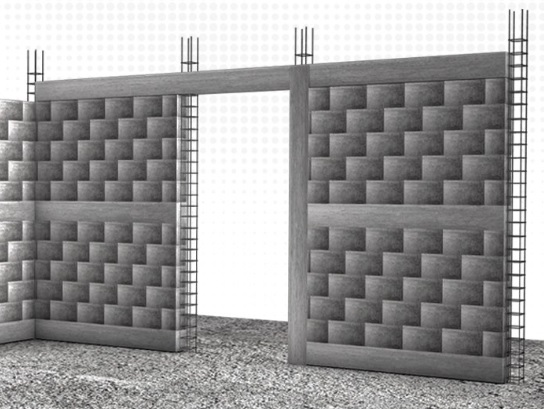
\includegraphics[width=0.6\textwidth]{mocheta1}
		\caption{Mocheta en mampostería reforzada}
	\end{figure}

	
	\subsection{Proceso constructivo de mochetas en mampostería}
	
	\subsubsection{Preparación y replanteo}
	Se trazan en obra las dimensiones de la mocheta, que normalmente coincide con el espesor del muro y un ancho de 10 a 30 cm. Se marcan las ubicaciones de refuerzos verticales, que deben alinearse con cimentaciones y soleras superiores. Se verifican los niveles y plomos para evitar desviaciones.  
	
	\subsubsection{Armado y refuerzo}
	Se colocan barras longitudinales en las celdas de bloque que formarán la mocheta.  
	- Para mochetas pequeñas: Ø 3/8” (\#3).  
	- Para mochetas de jamba: Ø 1/2” (\#4) o superior, dependiendo del cálculo.  
	El refuerzo debe anclarse en la cimentación y tener traslapo en la solera superior. Se recomienda usar amarres transversales o ganchos a 90° para integrarse mejor con el muro.  
	
	
	\subsubsection{Levantado de la mocheta}
	Se colocan bloques o ladrillos de forma alternada, cuidando la trabazón con el muro. En cada 40–60 cm de altura, se alinean las juntas verticales con las barras de acero. Las celdas con acero se rellenan con concreto fluido de  $f'_{c} \geq 210 \,\text{kg/cm}^2$, recomendado por la NSE 7.4. Se vibra o varilla el relleno para evitar vacíos.  
	
	\begin{figure}[h]
		\centering
		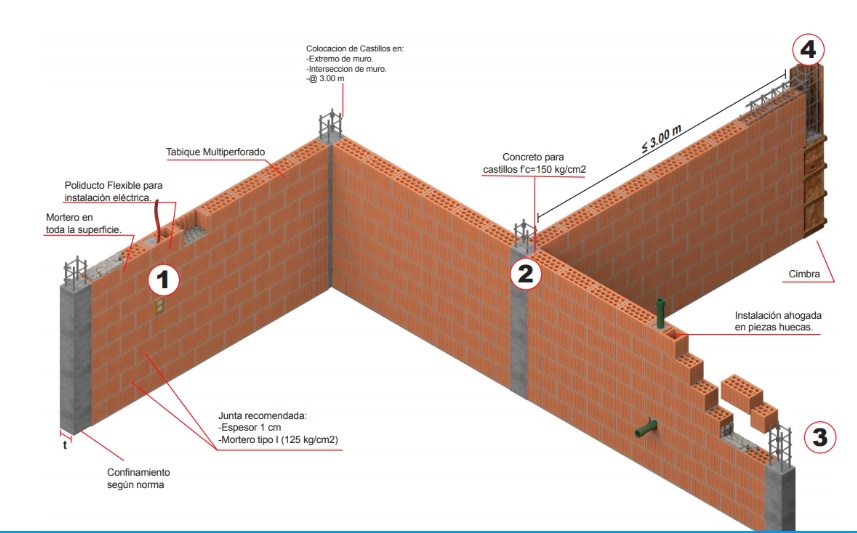
\includegraphics[width=0.6\textwidth]{mocheta3}
		\caption{Distribución de mochetas}
	\end{figure}
	
	\subsubsection{Instalación de soleras y confinamiento}
	Una vez alcanzada la altura del vano o techo, se coloca una solera de concreto armado, que amarra la mocheta con el muro. Si la mocheta está junto a un vano, se conecta con el dintel, formando un marco de confinamiento.  
	
	\subsubsection{Curado}
	El mortero de pega debe mantenerse húmedo al menos durante 3 días, cubriéndose con plásticos o regando periódicamente.  
	El concreto colado en las celdas y soleras debe curarse según ACI 308R:  
	- Mantenerlo húmedo durante 7 días.  
	- En climas cálidos y secos (ej. oriente de Guatemala), usar membranas de curado para evitar evaporación rápida.  
	- En el altiplano frío (ej. Quetzaltenango), controlar el curado para evitar fisuración por baja temperatura nocturna.  
	
	\subsection{Instalación y coordinación}
	Las mochetas deben levantarse de forma solidaria al muro, asegurando que no queden juntas frías. Se deben prever ductos o cajas eléctricas dentro de la mocheta si pasan instalaciones. Se controla la verticalidad y el aplome en cada hilada. En proyectos sismo-resistentes, las mochetas deben estar amarradas a la estructura principal mediante soleras, castillos y refuerzos continuos.  
	
	\subsection{Ventajas y desventajas}
	
	\subsubsection{Ventajas}
	- \textbf{Resistencia}: incrementan la capacidad portante del muro.  
	- \textbf{Confinamiento sísmico}: según NSE 7.4, mejoran el comportamiento ante cargas laterales.  
	- \textbf{Integración arquitectónica}: sirven como acabado de vanos, ocultando imperfecciones.  
	- \textbf{Durabilidad}: con buen curado y protección, son altamente resistentes al desgaste.  
	- \textbf{Versatilidad}: se adaptan a diferentes anchos y materiales de mampostería.  
	
	\subsubsection{Desventajas}
	- \textbf{Costo adicional}: requieren acero, concreto y mano de obra calificada.  
	- \textbf{Tiempo de ejecución}: demanda mayor planificación que un muro simple.  
	- \textbf{Fisuración}: si no se curan correctamente, aparecen grietas longitudinales.  
	- \textbf{Rigidez excesiva}: pueden generar concentraciones de esfuerzos si no están bien integradas al muro.  
	- \textbf{Limitación en remodelaciones}: dificultan hacer nuevas aberturas.  
	

	\section{Solera}
	\subsection{Descripción general}
	
	La \textbf{solera} es un elemento lineal de concreto reforzado de baja altura, construido generalmente sobre el terreno natural o sobre la base de una estructura, con la función principal de servir como elemento de confinamiento, borde o apoyo para pisos, banquetas, muros o cierres perimetrales. También puede actuar como transición entre niveles de piso, apoyo de marcos metálicos o borde de pavimentos.
	
	Las soleras pueden ser \textit{corridas} (a lo largo de muros o cerramientos), o \textit{aisladas} (de arranque o confinamiento). Su resistencia y dimensiones varían según el uso, pero normalmente presentan alturas entre 10 y 20 cm y un ancho de 15 a 30 cm.
	
	\subsection{Proceso constructivo de soleras}
	
	\begin{enumerate}[label=\textbf{\arabic*.},leftmargin=1.2cm]
		\item \textbf{Trazado y nivelación.}  
		Se marcan los ejes, alineaciones y cotas del nivel de solera. Se revisa la compactación del terreno o subbase donde apoyará el concreto, verificando que tenga la densidad y humedad adecuadas.
		
		\item \textbf{Encofrado (cimbra).}  
		Se instalan las tablas o formaletas laterales, perfectamente alineadas y firmemente sujetas. Se debe revisar la nivelación longitudinal y transversal, así como el espesor uniforme de la solera. Es común emplear madera cepillada o láminas metálicas en tramos rectos.
		
		\item \textbf{Armado.}  
		Según el diseño estructural o de refuerzo mínimo, se colocan varillas longitudinales (normalmente \#3 o \#4) y estribos cerrados o semicerrados con separación de 20 a 25 cm. Se asegura el recubrimiento mínimo (2.5 cm si está en contacto con el terreno, 4 cm si hay humedad permanente).
		
		\item \textbf{Instalaciones embebidas.}  
		Antes del vaciado se colocan ductos eléctricos, drenajes o anclajes metálicos, garantizando su alineación y protección.
		
		\item \textbf{Colado del concreto.}  
		Se vierte el concreto (f’c 210–280 kg/cm\textsuperscript{2}), compactando con varilla o vibrador de aguja corto. Se evita la segregación y se nivela con regla metálica o madera. El acabado puede ser liso, escobillado o rugoso, según el uso.
		
		\item \textbf{Curado.}  
		Se inicia dentro de las primeras horas posteriores al fraguado, manteniendo la superficie húmeda mediante riego constante o cubriendo con plástico/manta húmeda durante al menos 7 días.
		
		\item \textbf{Desencofrado y limpieza.}  
		Las formaletas se retiran después de 24 a 48 horas, cuando el concreto tenga resistencia suficiente. Se limpia el frente y se revisan defectos o nidos de grava.
	\end{enumerate}
	
	\subsection{Ventajas y desventajas}
	\begin{itemize}
		\item \textbf{Ventajas:} elemento económico, fácil de ejecutar, buena durabilidad y resistencia ante cargas ligeras; permite corregir desniveles o actuar como tope estructural.
		\item \textbf{Desventajas:} susceptible a agrietarse si el suelo no está bien compactado o si no se realiza un buen curado; requiere control de niveles y juntas de dilatación en tramos largos.
	\end{itemize}
	
	\subsection{Checklist de supervisión de soleras}
	
	\begin{tabularx}{\linewidth}{>{\raggedright\arraybackslash}p{0.64\linewidth} >{\centering\arraybackslash}m{1.5cm} >{\raggedright\arraybackslash}p{2.6cm} >{\centering\arraybackslash}m{2cm} >{\centering\arraybackslash}m{2.2cm}}
		\toprule
		\textbf{Actividad a revisar / ordenar} & \textbf{Estado} & \textbf{Responsable} & \textbf{Hora} & \textbf{Firma}\\
		\midrule
		Revisión de \textbf{planos y cotas de nivel} antes del trazo. & \cbox & & & \\
		Compactación y humedad del terreno o subbase verificadas. & \cbox & & & \\
		Formaletas alineadas, firmes y niveladas (sin fugas). & \cbox & & & \\
		Aplicación ligera de \textbf{desmoldante} en las tablas laterales. & \cbox & & & \\
		Colocación de acero (varillas y estribos) conforme planos y recubrimientos. & \cbox & & & \\
		Instalaciones (eléctricas, drenaje, anclajes) fijadas y protegidas. & \cbox & & & \\
		Concreto con la \textbf{resistencia f’c especificada}, revenimiento adecuado. & \cbox & & & \\
		Compactación con varilla o vibrador ligero sin segregación. & \cbox & & & \\
		Nivelación y acabado superficial uniforme. & \cbox & & & \\
		Inicio de curado dentro de 2 horas posteriores al colado. & \cbox & & & \\
		Curado continuo por mínimo de 7 días o según especificación. & \cbox & & & \\
		Retiro de formaletas cuando el concreto no se dañe. & \cbox & & & \\
		Revisión final de \textbf{fisuras, bordes y acabado}. & \cbox & & & \\
		\bottomrule
	\end{tabularx}
	

	\section{Vigas}
	\subsection{Descripción general}
	
	Las \textbf{vigas de concreto reforzado} son elementos estructurales lineales cuya función principal es resistir cargas verticales (flexión, cortante y torsión) y transmitirlas a los apoyos o columnas. Pueden ser vigas de entrepiso, de cimentación, de corona o de amarre, y su diseño depende de las luces, cargas y características del sistema estructural.
	
	Las vigas suelen ejecutarse in situ junto con las losas o en elementos prefabricados. En obra tradicional, se cimbran y refuerzan simultáneamente con losas y columnas.
	
	\subsection{Proceso constructivo de vigas}
	
	\begin{enumerate}[label=\textbf{\arabic*.},leftmargin=1.2cm]
		\item \textbf{Trazado y nivelación.}  
		Se definen ejes y cotas de nivel de vigas según los planos estructurales. Se revisa que los apoyos (columnas o muros) estén correctamente alineados y nivelados.
		
		\item \textbf{Encofrado (cimbra).}  
		Se instalan las formaletas laterales y el fondo de la viga, asegurando una correcta alineación, nivel y rigidez. Las juntas se sellan para evitar fugas de lechada.  
		Es fundamental que la cimbra soporte el peso del concreto fresco y del personal, utilizando apuntalamientos y contraventeos adecuados.  
		En vigas coladas junto con losas, el fondo se cimbrará junto con la losa y los laterales se ajustan con precisión al eje y peralte indicado en planos.
		
		\item \textbf{Armado.}  
		Se colocan las barras longitudinales principales (inferiores y superiores), los estribos y anclajes conforme a planos.  
		El recubrimiento mínimo debe ser de 2.5 cm (si está protegida) o 4 cm (si expuesta).  
		Los estribos se amarran a las barras principales con alambre recocido, cuidando la separación y posición según diseño.  
		Se colocan \textbf{ganchos de anclaje} en extremos y refuerzos adicionales en zonas de apoyo y continuidad con las losas.
		
		\item \textbf{Instalaciones embebidas.}  
		Se revisa que no existan interferencias con ductos eléctricos o tuberías. Los huecos deben estar aprobados por el ingeniero supervisor.
		
		\item \textbf{Colado.}  
		Se vierte el concreto (f’c 280 kg/cm\textsuperscript{2} típico en vigas estructurales), cuidando la compactación con vibrador de aguja y evitando la segregación.  
		En caso de colado conjunto con la losa, se garantiza la continuidad del refuerzo y un correcto vibrado en la interfaz losa–viga.
		
		\item \textbf{Curado.}  
		Una vez realizado el acabado, se inicia el curado mediante riego, mantas húmedas o aplicación de membrana. El curado debe mantenerse por al menos 7 días para prevenir fisuración y pérdida de resistencia.
		
		\item \textbf{Descimbrado.}  
		El retiro de la cimbra lateral se realiza cuando el concreto alcance una resistencia mínima que permita no dañar los cantos.  
		Los apuntalamientos del fondo se retiran solo cuando el concreto alcance la resistencia especificada por el diseño o según los tiempos de fraguado determinados por el supervisor.
	\end{enumerate}
	
	\subsection{Ventajas y desventajas}
	\begin{itemize}
		\item \textbf{Ventajas:} excelente capacidad estructural, permite claros medianos y largos, se integra fácilmente con columnas y losas, y brinda rigidez lateral a la estructura.  
		\item \textbf{Desventajas:} requiere cimbra robusta, mayor tiempo de ejecución y control estricto de niveles, vibrado y curado para evitar deflexiones o grietas.
	\end{itemize}
	

	
	

	
			

		
	
	  
	
	
	
	
			

\end{document}
